\subsection{Constant source diffusion (Predeposition)}

Although the diffusion process of donors and acceptors into the silicon crystal is a three dimensional process for simplicity we first only discuss the one dimensional mathematics for it in order to get a "simple" equation for the depth-time-temperature relation.

\begin{mdframed}[linewidth=2pt,linecolor=red]
This is only valid for a constant source of dopants on the surface of the wafer (gas, for instance).
These equations are used for predicting the pre-deposition step (in case this process would be adapted by someone for predeposition instead of ion implant)
\end{mdframed}

We start with Ficks\footnote{\url{https://en.wikipedia.org/wiki/Fick\%27s_laws_of_diffusion}} law (for all German speakers: Yes that's his name) where the dopant concentration N is coupled with time and place
\begin{equation}
\frac{\partial N}{\partial t} = D \cdot \frac{\partial^2 N}{\partial x^2}
\end{equation}

The diffusion coefficient is as well material as well as temperature dependent  and can be calculated with the following equation:
\begin{equation}
D = D_0 \cdot \exp\left(-\frac{E_a}{k \cdot T}\right)
\end{equation}
With $k=8.62 \cdot 10^{-5} \frac{eV}{K}$ being the Boltzman constant and in table \ref{table:absolute_diffusion_coefficients} we can see the $D_0$ and $E_a$ values for the most common materials\footnote{ISBN 3-8023-1588:Hoppe Bernhard, Mikroelektronik 2, Page 24, Table 2.1} which we can use within the further calculations for our well dimensioning phases. The temperature usually is in the area of $1000\degree C$ or $1273.15 K$.
\begin{table}[H]
	\label{table:absolute_diffusion_coefficients}
	\centering
	\begin{tabular}{|c|c|c|}
		\hline
		Element &
		$D_0$ $\left[\frac{cm^2}{s}\right]$ &
		$E_a$ $\left[eV\right]$ \\
		\hline
		P &
		10.50 &
		3.69 \\
		\hline
		As &
		0.32 &
		3.56 \\
		\hline
		Sb &
		5.60 &
		3.95 \\
		\hline
		B &
		10.50 &
		3.69 \\
		\hline
		Al &
		8.00 &
		3.47 \\
		\hline
		Ga &
		3.60 &
		3.51 \\
		\hline
		Cu &
		0.0025 &
		0.65 \\
		\hline
	\end{tabular}
	\caption{$D_0$ and $E_a$ values for boron and phosphorus}
\end{table}

The law stated above
\begin{equation}
\frac{\partial N}{\partial t} = D \cdot \frac{\partial^2 N}{\partial x^2} 
\end{equation}
has the same form as the temperature conductivity equation (Laplace) for which we already have a general solution
\begin{equation}
\frac{\partial u}{\partial t} = a^2 \cdot \frac{\partial^2 u}{\partial x^2} 
\end{equation}

Which means that we can map the general solution for the temperature conductivity equations after Laplace
\begin{equation}
u(x,t) = \frac{1}{2 \cdot a \cdot \sqrt{\pi \cdot t}} \cdot \int_{-\infty}^{\infty}{f(a)\cdot\exp\left(\frac{-(x-a)^2}{4 \cdot a^2 \cdot t^2}\right)}da
\end{equation}
to our Ficks law with $a=\sqrt{D}$ and $u=N$
\begin{equation}
N(x,t) = \frac{1}{2 \cdot \sqrt{D} \cdot \sqrt{\pi \cdot t}} \cdot \int_{-\infty}^{\infty}{f(\sqrt{D})\cdot\exp\left(\frac{-(x-\sqrt{D})^2}{4 \cdot D \cdot t^2}\right)}da
\label{eq:ficks_law_expanded}
\end{equation}
with the edge conditions
\begin{equation}
N( x=0 , t > 0 ) = N_0
\end{equation}
\begin{equation}
N( x \geq 0 ,  t = 0 ) = 0
\end{equation}
we get the resulting function from the solving process for the Laplace temperature conduction equations
\begin{equation}
u(x,t)=u_0 \cdot erfc\left(\frac{x}{2 \cdot a \cdot \sqrt{t}}\right)
\end{equation}
with the error function being an integral of the form
\begin{equation}
erfc(z)
=
\left(1-\frac{2}{\sqrt{\pi}}\right)\cdot\int_0^z{e^{-a^2}}da
\end{equation}

Or in case of our dopant concentration equation we can replace a with the square root of the diffusion coefficient in order to get the error function for our dopant density equation:
\begin{equation}
erfc(z)
=
\left(1-\frac{2}{\sqrt{\pi}}\right)\cdot\int_0^z{e^{-D}}d\sqrt{D}
\end{equation}
\begin{equation}
N(x,t)
=
N_0 \cdot erfc\left(\frac{x}{2 \cdot \sqrt{D \cdot t}}\right)
=
N_0 \cdot erfc\left(\frac{x}{x_l(t)}\right)
\end{equation}
Now we can extract the layer thickness and the depth of the well in dependency of the time and the temperature, respectively:
\begin{equation}
x_l(t) = 2 \cdot \sqrt{D \cdot t}
\end{equation}
\begin{equation}
x_l(t) = 2 \cdot \sqrt{D_0 \cdot \exp\left(-\frac{E_a}{k \cdot T}\right) \cdot t}
\end{equation}

And plot the result for multiple different drive in times
\begin{figure}[H]
	\centering
	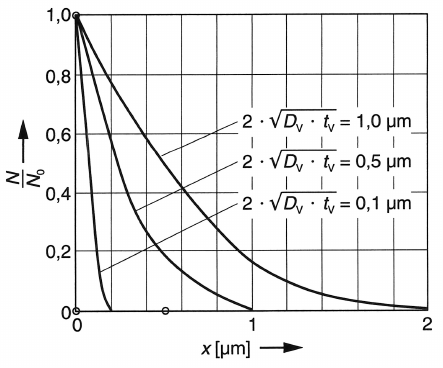
\includegraphics[scale=0.5]{dopants_depth.png}
	\caption{Different predeposition times}
\end{figure}

We can now describe the dosage based on the time and temperature of the diffusion

\begin{equation}
Q=\frac{2}{\sqrt{\pi}} \cdot N_0 \cdot \sqrt{D \cdot t}
\end{equation}

Where $N_0$ (concentration at the surface) equals the maximum solubility of a given element (e.g. boron) within the given medium (e.g. silicon).\footnote{If someone really wants to do this in his basement he can google these values and make a pull request}
